%\documentclass[a4paper,9pt,fleqn,notoc]{diss}
%%\renewcommand{\includegraphics}[1][1]{}
%\begin{document}

\chapter{Function and Evolution of Locative Spatial Grammar}
\label{s:grammar}
Purely lexical communication systems are limited
because while they enable agents to express semantic entities, in a restricted sense 
they do not allow to encode how these semantic entities are supposed to be used,
in particular, they do not encode how to process the spatial context.
For instance, the following three utterances 

\begin{example}
\label{e:der-linke-block}
\gll der linke Block 
the.NOM left.ADJ.NOM block.NOM 
\glt `The left block',
\glend
\end{example}
\begin{example}
\label{e:links-des-blockes}
\gll links des Blockes
left.PREP.GEN the.DET.GEN block.GEN 
\glt `to the left of the block',
\glend
\end{example}
and
\begin{example}
\label{e:der-block-links}
\gll der Block links
the.DET.NOM block.NOM left.ADV
\glt `the block to the left',
\glend
\end{example}
all consist of the same lexical material but their meaning structure is quite different.
In Example \ref{e:der-linke-block} the spatial relation is used as modifier on the set of
objects denoted by the noun, whereas in Example \ref{e:links-des-blockes} the
spatial category is applied to a landmark denoted by the noun. In Example \ref{e:der-block-links}
a determined noun phrase is followed by the category expressed as an adverb which
denotes a region that is used to modify the set of blocks. In difference to Example \ref{e:der-linke-block}, 
however, the spatial category is related to a covert landmark, not a 
group-based relative reference system.
If an agent in a spatial language game is confronted with these utterances, he is supposed to 
process the context differently in each case. In some contexts the referent
denoted by each of these two utterances might be the same, but this is not necessarily
true for all spatial scenes. Clues for the different processing of these
utterances are in the grammatical structure of each of them. In the first case, 
the word order and the
morphology make it clear that the spatial category is used as an adjective within a
determined adjective noun phrase. In the second case, it is the usage of the spatial
category as preposition that encodes that the determined noun phrase tail of the phrase
is denoting the landmark to which the spatial relation is applied. 
In Example \ref{e:der-block-links}, the lack of a following noun phrase reveals the use of the spatial category as 
adverb which entails inferences about the type of the region, e.g., the region can be internal or external 
and there must be a covert landmark. Consequently, these three examples show how the German grammatical 
system provides valuable indications as to how to interpret each of these utterances.
In this chapter, I will be concerned with two claims following from this observation. First,
grammar is necessary to avoid ambiguity and errors in interpretation. Second, given the
communicative need to avoid such problems in communication, agents equipped with
the right learning and invention operators can develop grammatical communication systems\footnote{Ideas and results presented in this chapter are 
published in \citep{spranger2012grammar}\index{Spranger, M.} and \citep{spranger2010space}\index{Loetzsch, M.}\index{Pauw, S.}\index{Spranger, M.}.}.


\begin{figure}
\begin{center}
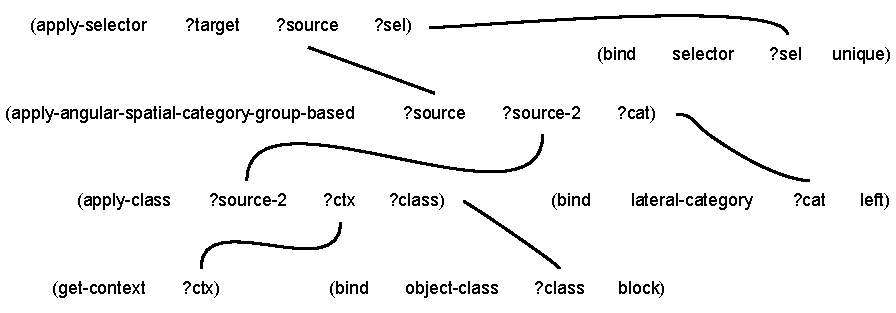
\includegraphics[width=1.0\columnwidth]{figs/semantic-structure-der-linke-block}
\end{center}
\caption[Semantic structure example spatial adjective]{Semantic structure underlying Examples \ref{e:der-linke-block} and \ref{e:linke-block-der}. 
The semantic structure has three semantic entities which are linked in such a way that
the set of blocks filtered by the primitive {\footnotesize\tt apply-class} is further
filtered by the spatial category {\footnotesize\tt left} which is applied here to a group-based 
relative landmark. Finally, the selector {\footnotesize\tt unique} is applied retrieving the 
best scoring element.}
\label{f:semantic-structure-1}
\end{figure}

\begin{figure}
\begin{center}
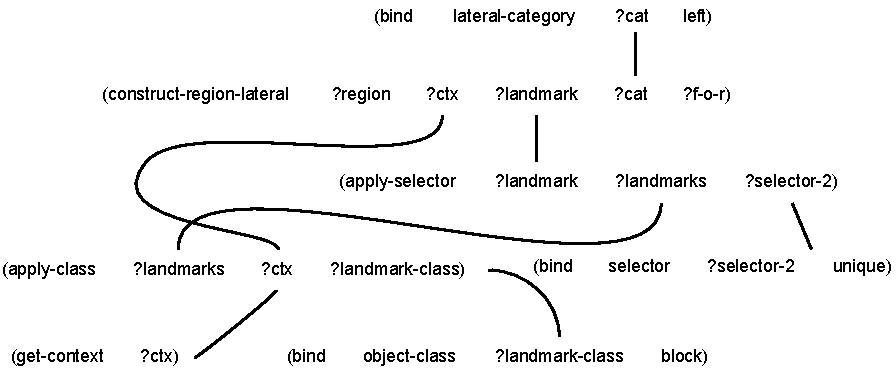
\includegraphics[width=1.0\columnwidth]{figs/semantic-structure-links-des-blockes}
\end{center}
\caption[Semantic structure example lateral region with landmark]{
Semantic structure underlying Examples \ref{e:links-des-blockes}
and \ref{e:linke-block-der}. This semantic structure encodes how to construct
a lateral region based on the spatial relation {\footnotesize\tt left} using the landmark 
that is provided by the subpart of the structure singeling out an object from the context
by applying the object class {\footnotesize\tt block} and the selector {\footnotesize\tt unique}.}
\label{f:semantic-structure-2}
\end{figure}
\begin{figure}
\begin{center}
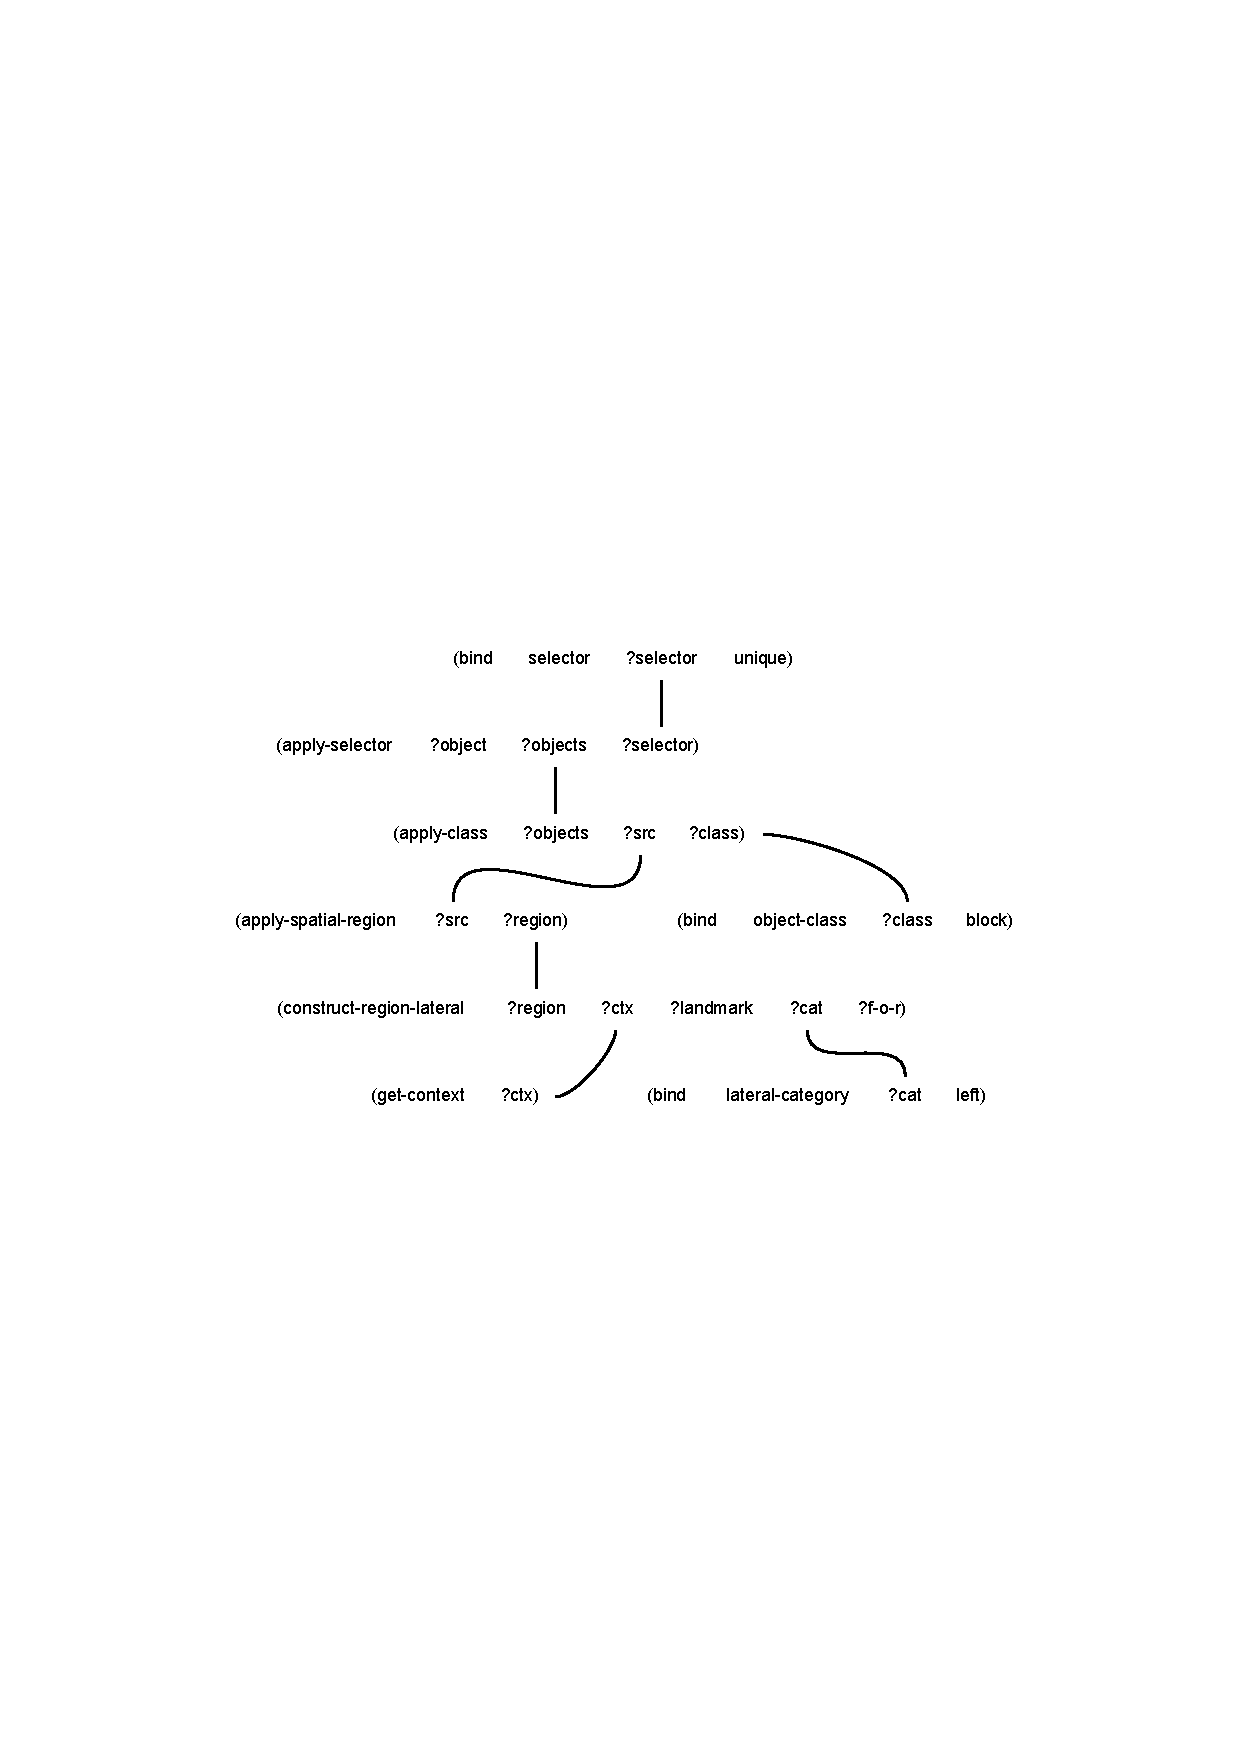
\includegraphics[width=1.0\columnwidth]{figs/semantic-structure-der-block-links}
\end{center}
\caption[Semantic structure example lateral region without landmark]{Semantic structure underlying 
Example \ref{e:der-block-links} and \ref{e:linke-block-der}. 
The spatial relation {\footnotesize\tt left} is used here to construct a
region based on an unspecified landmark. The region is used to filter the context,
followed by the application of the object class {\footnotesize\tt block} to further filter the objects,
followed by the application of the selector {\footnotesize\tt unique}.}
\label{f:semantic-structure-3}
\label{f:semantic-structure}
\end{figure}


\section{The Importance of Grammar}
The main hypothesis pursued in this section is that grammar is important because it 
conveys information as to how lexical items, e.g. spatial relations, interact in semantic structure
and which role the lexical items play within the semantic structure. 
By providing this important information on how to process the context,
grammar reduces the search space of possible interpretations of a phrase and 
thereby enhances the communicative success\index{measures!communicative success} of the population.
To see this, it is helpful to consider what is left if one were to ``remove'' the 
grammatical cues from Examples \ref{e:der-linke-block} to \ref{e:der-block-links}.
In principle, one ends up with a phrase like the following.
\begin{example}
\label{e:linke-block-der}
\gll link block der
left block the
\glt
\glend
\end{example}
This phrase is non-grammatical because it lacks proper German morphology
and word order among other things. Now this phrase can 
be interpreted in many different ways. 
Since semantics are represented using IRL, we
will immediately make this point using IRL-networks 
to formalize what is meant by different 
semantics. Three plausible spatial semantic interpretations 
of Example \ref{e:linke-block-der} are 
shown in Figures \ref{f:semantic-structure-1}, 
\ref{f:semantic-structure-2} and \ref{f:semantic-structure-3}.
The semantic structures shown in these figures formalize 
the intuitive notions formulated
in the beginning of this chapter as to what the difference is in 
the semantics of Examples \ref{e:der-linke-block} to \ref{e:der-block-links}
which are all utterances built using the same lexical material as Example \ref{e:linke-block-der}.
Mort importantly, however, all three semantic structures are valid interpretations of 
Example \ref{e:linke-block-der} because Example  \ref{e:linke-block-der} 
only constraints the space of possible interpretations by providing
a set of semantic entities that need to be part of the semantic structure. The three 
semantic entities encoded in this utterance are part of all three semantic structures. 
To understand then what information grammar
provides in the formal framework of IRL, 
one can examine the differences in interpretations. 
There are two important differences 
between these structures; the first is related to the cognitive
operations involved. For instance, semantic structure \ref{f:semantic-structure-1}
involves the operation {\footnotesize\tt apply-spatial-category-group-based} 
which is not found in
\ref{f:semantic-structure-2} or \ref{f:semantic-structure-3}. The other 
important difference is in terms of how operations are linked. The 
difference between the structures in Figures \ref{f:semantic-structure-2}
and \ref{f:semantic-structure-3} is not only which cognitive operations 
are part of each of them, but primarily one of how the cognitive 
operations are linked. In Figure \ref{f:semantic-structure-2},
the landmark of the spatial region is given by the subnetwork consisting 
of {\footnotesize\tt apply-selector} and {\footnotesize\tt apply-class}, whereas in 
\ref{f:semantic-structure-3} this subnetwork is linked to the output of
the operation {\footnotesize\tt apply-spatial-region} so as to further refine the 
set of objects which are filtered using the spatial region. In the formal 
framework pursued in this book, grammar is related to which cognitive 
operations are part of the semantic structure of an 
utterance and how the semantic structure is internally linked.

\begin{figure}
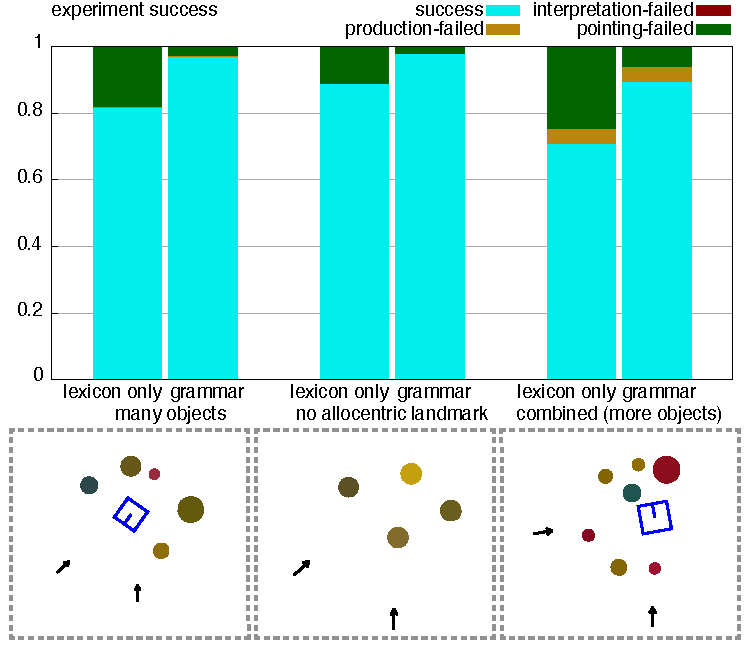
\includegraphics[width=1.0\columnwidth]{figs/why-grammar-german}
\caption[German locative phrases with and without grammar]{
The figure compares
the performance of agents equipped with a purely 
lexical system with a population in 
which all agents operate the German space 
grammar discussed in Section 
\ref{s:german-locative-phrases-syntax}.
There are three conditions \emph{many objects}, 
\emph{no allocentric landmark} and 
\emph{combined (more objects)}. In the first 
condition, agents have similar perspectives on the scene 
and there are quite a few objects. In the middle condition, there 
is no box landmark. Agents can only use 
themselves as landmark or have to resort to group-based 
reference. The last condition is a combination
of the two, but with scenes that have even more objects.}
\label{f:why-grammar-german}
\end{figure}


\begin{figure}
\begin{center}
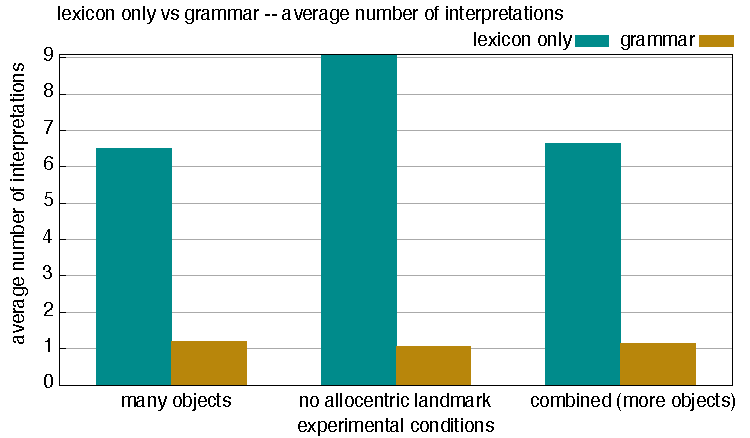
\includegraphics[width=0.9\columnwidth]{figs/why-grammar-german-avg-interpretations}
\end{center}
\caption[Comparison average number of interpretations]{\index{measures!average number of interpretations}
This figure compares the number of semantic 
structures tried in interpretation for German locative 
phrases processed 
with and without grammar.}
\label{f:why-grammar-german-interpretation-1}
\end{figure}

\begin{figure}
\begin{center}
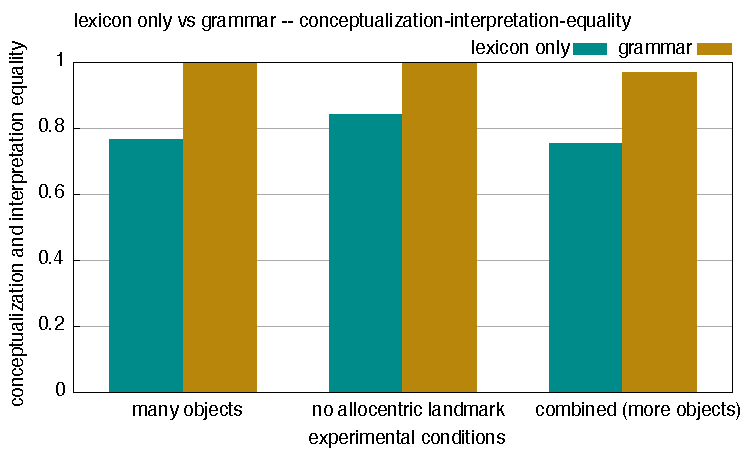
\includegraphics[width=1.0\columnwidth]{figs/why-grammar-conceptualization-interpretation-equality}
\caption[Comparison interpretation equality]{
This figure shows how similar the semantic structure 
recovered by the hearer is to the conceptualization strategy of 
the speaker. The effect is compared for different sets of spatial scenes. 
If the semantic structures are equal, the interaction counts as 1.0, if 
not -- as 0.0. The results show the average over 10000 interactions. 
In the case of grammatical systems, the speaker was able to recover the correct semantic structure
in all games. For purely lexical systems this number drops to 80\%. This number correlates
to some respect with communicative success\index{measures!communicative success}. But not in all spatial scenes is a drop 
in the number of scenes in which the hearer correctly interprets the phrase equal to
to a drop in communicative success.}
\label{f:why-grammar-german-interpretation-2}
\end{center}
\end{figure}

Removing the grammatical cues from 
Examples \ref{e:der-linke-block} to \ref{e:der-block-links}
increases the number of possible interpretations of these phrases.
Consequently, grammar is related to semantic 
ambiguity which I defined as different possible semantic structures \index{measures!average number of interpretations}underlying the 
same utterance (see Section \ref{s:semantic-ambiguity}). 
The increase in possible interpretations of a phrase
impacts in two ways. First, it can lead to failure in communication 
because the hearer interprets the phrase differently and the different 
interpretation leads to mistakes in 
establishing reference, i.e., the hearer interprets the phrase to refer to the wrong
topic. Second, semantic ambiguity\index{semantic ambiguity} leads to additional 
effort in interpretation on the part of the hearer. If there are multiple interpretations, of 
a phrase, the hearer has to test all of them in order to find the correct interpretation.

\subsection{Experimental Results}
Figure \ref{f:why-grammar-german} shows what happens when all 
grammatical constructions are removed from the German locative 
system. Every utterance produced by an agent operating a lexical 
system conveys only the semantic entities, e.g. spatial relations, 
object classes, determiners and discourse roles without explicitly 
marking their relationships in the semantic structure. Figure 
\ref{f:why-grammar-german} compares the performance on different 
sets of spatial scenes with varying features and degrees of complexity. 
To the left the condition is one in which many objects are distributed 
around an allocentric landmark. The middle condition is one in which 
scenes have no allocentric landmark. The condition 
shown to the right has both scenes with allocentric and 
without allocentric landmark but is generally more complex with 
respect to the number of objects and distribution of objects. 
Additionally, the position of the interlocutors is more varied. Clearly, the more complex 
spatial scenes are the more important non-ambiguous communication is. On the other hand, 
it is quite strikingly not the case that communication breaks down completely when agents are lacking grammatical devices in their language. Rather, agents are in general successful in communication. 
They are able to establish correct reference in well over 70\% of cases and, for instance in the middle condition in almost 90\% of the cases. 
The reasons for this is the powerful active interpretation capacity that agents are
endowed with which allows them to find the most probable object given the 
lexical material they observe in the utterance. But this success is also in part 
due to the overall limited nature of conceptualization strategies which for every 
scene is among the range of 10 but not infinitely large which allows agents to guess 
the meaning of purely lexical utterances.

Clearly, there is a communicative 
advantage for having grammatical constructions that allow agents to recover
additional information not communicated by lexical items alone.
Figure \ref{f:why-grammar-german-interpretation-1} shows the advantage of grammar 
in processing spatial utterances by comparing the number
of interpretations hearers had to try in order to arrive at the best interpretation
of the phrase. This number is significantly higher for lexical systems than it is 
for the German locative grammar discussed in this book. 
Essentially the results measure semantic ambiguity\index{semantic ambiguity} and show efficiency 
in interpreting utterances. The figure shows the average number 
of interpretations (10000 interactions). In the case of grammar, the 
average is just barely above 1.0. When agents are equipped 
with grammar, there is only one type of utterance that is really 
ambiguous in terms of processing. An example of such an utterance 
is ``der Block links der Kiste'' (the block left of the box),
which can be interpreted in an intrinsic or relative way. For purely 
lexical systems the number of interpretations the hearer has to try for 
each phrase is high. On average more than six interpretations have 
to be tried for every single utterance in all three conditions. The peak 
for the condition \emph{no allocentric landmark} is due to the 
increased number of utterances consisting of three lexical 
items in this condition. Utterances involving three lexical items can 
be interpreted as determined adjective noun phrases, but also in many 
ways including covert spatial landmarks and even perspective.
The middle condition licenses many three word utterances. Because of the 
lack of an allocentric landmark, speakers will often choose the adjectival 
strategy without being able to clearly express themselves and mark 
their strategy using grammar. Nevertheless, if we look back at the 
impact on communicative success, there is no direct correlation 
between number of interpretations of a phrase
and communicative success. In the \emph{no allocentric landmark} 
condition the drop in success is not as strong as the rise in number 
of interpretations per phrase. An explanation can be seen in Figure 
\ref{f:why-grammar-german-interpretation-2}
which shows that while the number of interpretations increases, the 
rate with which hearers find the correct interpretation does not 
drop as strong for the condition.\index{measures!conceptualization-intepretation equality}

\subsection{Factors Influencing the Importance of Grammar}
If grammar has positive effects on processing and communicative success, 
one can ask the follow-up question: what are the factors determining
how much impact grammar has. How much agents with 
grammar perform better in terms of communicative success\index{measures!communicative success} is largely 
a function of the environment and the number of possible 
interpretations of each utterance. The more complex the environment 
and the larger the number of different possible interpretations of a phrase, 
the more problems occur in communication. If agents share similar viewpoints 
on the scene, if perceptual deviation is minimal and if there are only few objects 
in the scene, the effect of grammar is less strong 
than in cases where viewpoints are different, perceptual deviation is strong and the number of objects 
is high (a fact that is demonstrated in Figure \ref{f:why-grammar-german}). 
But these influences are quite subtle. For instance, the results shown in Figures
\ref{f:why-grammar-german-interpretation-1} and \ref{f:why-grammar-german-interpretation-2} suggest that it is not only the number of interpretations that make a difference, but the ambiguity has to matter with respect to the environment. for
instance, perspective is relevant to certain aspects of the German locative system,
but it does not necessarily cause problems in communication. Many conceptualization
strategies such as the absolute one are agnostic to perspective. One
also has to be careful not to confuse the sensitivity of some conceptualization strategies
with the impact of grammar. A strategy fully expressed in grammar can remain 
sensitive to perspective, e.g., determined spatial adjective noun phrases need to be 
interpreted with respect to some perspective. But the sensitivity remains if one expresses the
underlying group-based reference conceptualization strategy lexically only.

\index{measures!conceptualization-intepretation equality}\index{measures!average number of interpretations}
The performance with respect to processing is governed by the number of
possible different interpretations of a particular phrase. The higher the number of 
possible interpretations is the more conceptualization strategies need to be tested 
and processed. The number is essentially a function of how much re-use of 
lexical items occurs in the language or how much particular semantic entities 
such as spatial relations participate in different interpretations.
For instance, in the German locative system, lateral and frontal projective 
spatial relations occur in relative and intrinsic conceptualization strategies. 
Absolute categories do not participate in intrinsic and relative conceptualization 
strategies but only in absolute ones. To remove the power 
of grammar to disambiguate, therefore, has less effect on absolute spatial 
relations. Consequently, if a semantic entity only participates
in a single conceptualization strategy, removing parts of grammar related 
to that entity has little or no effect, whereas when the entity participates 
in many different conceptualization 
strategies this can have a big impact. Additionally, the increase in ambiguity is paired
with features of the environment. If features of the environment are such that agents 
are not using a particularly ambiguous set of strategies, than ambiguity 
does not play a role in these conditions.


\section{Emergence of Grammatical Markers}\index{grammatical marking}
Following the argument for the impact of grammar on communicative success 
and processing, I can turn to the question: what are the necessary 
invention, adoption and alignment mechanisms so that agents can self-organize grammatical communication systems? 
I will attempt to answer this question by looking at a smaller set of conceptualization strategies than the full-blown
German locative system and by reducing grammar deliberately to marking of conceptualization strategies. 
That is, I do not discuss how word order arises and may become shared or how the complex morphological system of German 
may be culturally negotiated. Rather, I look at grammatical systems that are 
marking the part of semantic structure related to processing of semantic entities. 
In this scheme, grammatical constructions map certain parts of semantic structure 
-- namely cognitive operations and their links to strings, henceforth called markers.
These constructions build up a shallow hierarchy. Their constituents are
 lexical items that provide semantic entities.

\begin{figure}
\begin{center}
%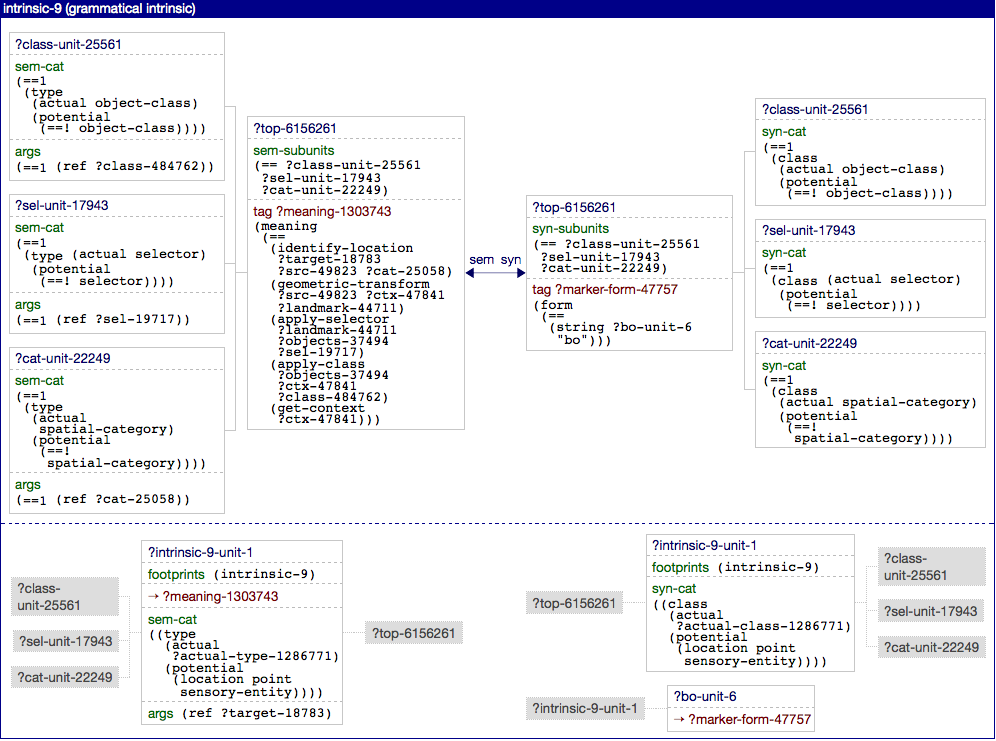
\includegraphics[height=0.58\columnwidth,angle=90]{figs/bo-construction}
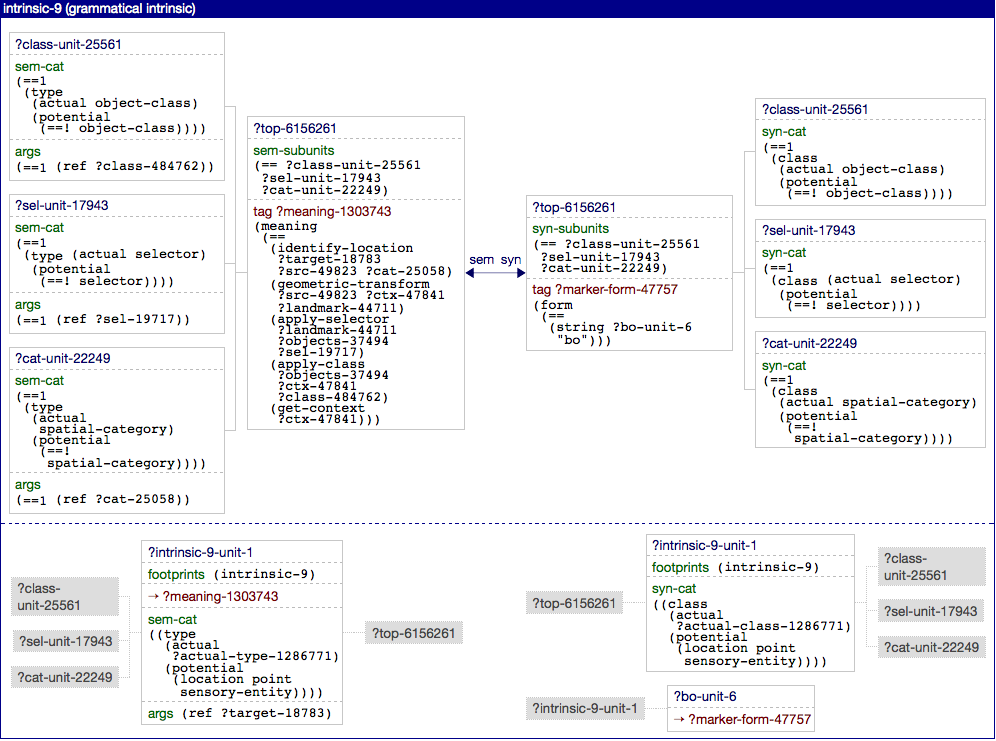
\includegraphics[width=0.98\columnwidth]{figs/bo-construction.png}
\end{center}
\caption[Example grammatical marker construction]{
Grammatical construction for marking the intrinsic conceptualization strategy
(see Figure \ref{f:semantic-structure-grammar-intrinsic}). The construction
has three lexical constituents: a spatial relation, a selector and an object class. In production,
the intrinsic strategy is expressed using the three lexical constituents plus the marker ``bo''
that is introduced by this construction. In parsing the construction fully recovers
the intrinsic conceptualization strategies upon observing three compatible lexical items 
and the marker ``bo''.
Notice that categories are the same on the syntactic and semantic side 
which follows the design of lexical constructions.}
\label{f:bo-construction}
\end{figure}

\begin{figure}
\begin{center}
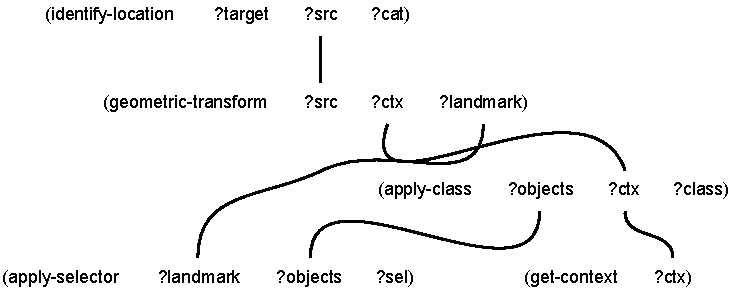
\includegraphics[width=0.9\columnwidth]{figs/semantic-structure-intrinsic-strategy-grammatical-marking}
\end{center}
\caption[Semantic structure intrinsic conceptualization strategy]{IRL-network of the intrinsic conceptualization strategy. A corresponding construction
for expressing this strategy is shown in Figure \ref{f:bo-construction}.}
\label{f:semantic-structure-grammar-intrinsic}
\end{figure}


An important example of semantic ambiguity\index{semantic ambiguity} in German locative phrases is related to
frames of reference. The lexical item ``\"uber'' (over) can
be processed in all three frames of reference: absolute, intrinsic and relative.
For studying the development of grammatical systems, agents are given four conceptualization
strategies: intrinsic, absolute, relative from the perspective of the speaker and relative
from the perspective of the hearer. Agents are equipped with four angular spatial relations, 
all of which are modeled after ``vor'' (front), ``hinter'' (back), ``links'' (left) and ``rechts'' (right) with the difference
that they behave like ``\"uber'' (up) and partake in intrinsic, relative and absolute conceptualization strategies. 
Agents operating only lexical constructions will express themselves always in three word
utterances. The utterances consist of the spatial relation as well as a determiner and a noun. 
All four strategies operate the same set spatial relations and all apply the frame of reference 
to an allocentric landmark which can be marked
lexically. For any utterance the three words alone never distinguish between the 
four conceptualization strategies given to
agents, but rather a hearer always has to try all four strategies, in order, to retrieve the most likely
topic. The lexical agents can be contrasted with agents operating grammatical constructions.
Grammatical constructions allow agents to communicate the conceptualization strategy they used
by marking it. Figure \ref{f:bo-construction} shows a grammatical construction that marks the intrinsic strategy  
(see Figure \ref{f:semantic-structure-grammar-intrinsic})
with the marker ``bo''. Consequently, an agent equipped with this construction,
if he uses the intrinsic strategy in conceptualization, constructs an utterance involving 
a spatial term, the determiner, an object class term and the marker ``bo''. Subsequently, in interpretation a hearer of this utterance parses a complete IRL-network and he is not required to additionally process the other conceptualization strategies to find the topic of 
the phrase. Figure \ref{f:why-grammar} compares the performance of lexical agents that 
only operate lexical constructions with agents that grammatically mark the 
conceptualization strategy they are using. We can observe similar effects of grammar 
both on processing and communicative success as for the complete
German locative system. Overall this justifies the simplified approach taken in this section.

\begin{figure}
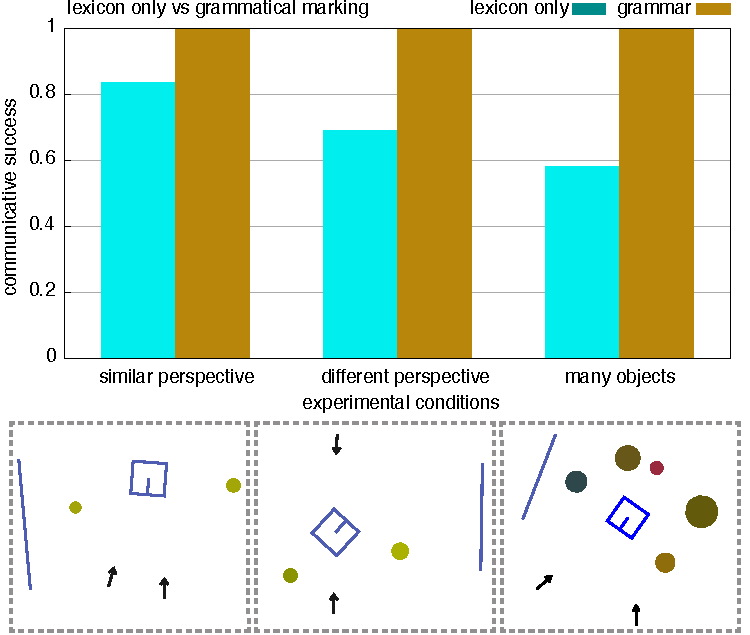
\includegraphics[width=1.0\columnwidth]{figs/why-grammar}
\caption[Comparison lexical versus grammatical agents]{
Comparison of purely lexical agents equipped with four angular 
conceptualization strategies. Half of the strategies are dependent on 
perspective, hence, the impact of changing the perspective of robots on the scene
is a major impact. Another factor is the number of objects in each scene.}
\label{f:why-grammar}
\end{figure}

\subsection{Invention and Alignment Operators}\index{alignment}
The results shown in this and the previous section undoubtedly demonstrate
the advantage of a communication system that allows agents to mark the usage 
of the same semantic entities in different conceptualization strategies. The clear 
communicative advantages for grammar in spatial settings can fuel a process whereby 
agents are actively developing grammatical markers in order to communicate more 
successfully. To verify this claim I research which diagnostics and repair 
strategies are needed for agents to invent grammatical constructions, and which 
alignment operations are needed so that agents develop a successful and concise 
grammatical system that helps them solve their communicative problems.

Invention and adoption of grammatical markers is implemented 
using dedicated diagnostics and repairs. Agents monitor themselves, 
diagnose problems and potentially repair 
diagnosed problems in communication.
When a speaker diagnoses that in production, particularly in re-entrance\index{re-entrance}, 
the utterance he is about to produce has multiple different topics, he 
creates a problem called \emph{multiple-target-entities}. 
This problem is fixed by a dedicated repair strategy that invents 
a grammatical construction. The new construction maps the semantic 
structure used in conceptualization onto a grammatical marker.
The speaker restarts production in the hope that the newly invented 
grammatical construction helps in disambiguating the conceptualization 
strategy he applied and, subsequently, reduces ambiguity in interpretation 
for the hearer. 
Upon hearing
the new marker, the hearer diagnoses the problem \emph{uncovered-strings} 
because he is exposed to the newly invented marker for the first time. The hearer 
in re-production invents a new grammatical construction mapping the 
observed unparsed string to the meaning he was able to re-conceptualize. 
At the end of the interaction both interacting agents have a grammatical 
construction that links the new marker to the conceptualization strategy both 
have used in production and re-production, respectively.

Besides invention and adoption, agents need alignment strategies. 
There are two goals for alignment strategies. First, the hearer might adopt 
the marker such that it links to a different conceptualization strategy then the 
one used by the speaker. In this case the alignment operators
have to orchestrate that one of the wrong mappings dies out over time. The 
second goal is that if there are multiple markers floating in the population 
for the same conceptualization strategy, then the agents of the population 
should come to an agreement as to which marker to use
for that particular strategy. Alignment for grammatical constructions is the same 
as for lexical constructions. Successfully used constructions are rewarded, unsuccessfully used constructions punished. Additionally, competitor 
constructions are punished; these are the constructions that could have 
been used in production but were not used because another construction 
covering the same semantic structure was applied and has a higher score. 
This of course implements \emph{lateral inhibition} dynamics for grammatical constructions. 


\subsection{Experimental Setup and Results}
The performance of the proposed invention, adoption and 
alignment operators is tested on different sets of spatial scenes. Agents are equipped 
with four spatial relations, one determiner and three object classes together 
with lexical constructions for expressing these items. In total
agents are given eight lexical constructions for the four spatial relations, the 
determiner and the three object classes (robot, box and block). Moreover, 
agents are given the four conceptualization strategies discussed earlier. The task for agent is then to develop a system that allows them to increase their success 
from the lexicon-only baseline condition to 100\% success. Figure 
\ref{f:why-grammar-development} shows the dynamics of development for 
populations operating the invention and alignment\index{alignment} operators as well as 
the lexical constructions and the semantic entities discussed. Agents are able 
to develop successful grammatical marking systems given the need 
to disambiguate semantic structure in all three environmental conditions considered. 
In all cases agents develop a grammatical marker system
consisting of four markers marking the four conceptualization strategies. 
We can also see that essentially in all conditions markers are necessary for disambiguation. It is just the number of contexts that require disambiguation 
that drives development of the marker system.
Clearly this number is low in the case of the \emph{similar perspective} condition.



\begin{figure}
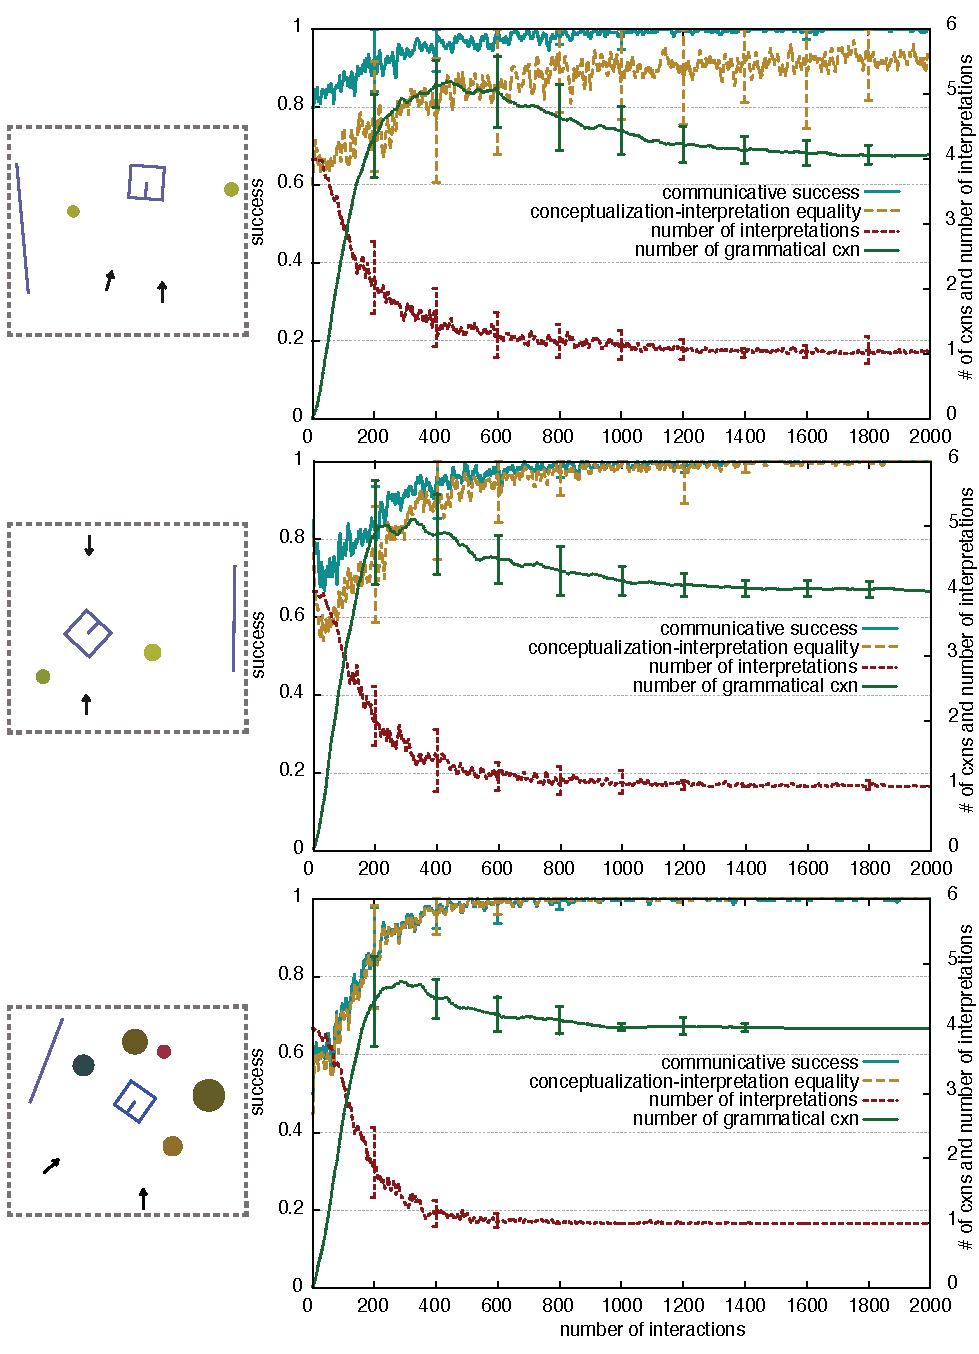
\includegraphics[width=0.9\columnwidth]{figs/why-grammar-development}
\caption[Development of grammatical markers over time]{Development of grammatical markers over time. As the number of 
grammatical markers in the population
increases, the number of interpretations per phrase drops. In all three
conditions agents self-organize a grammatical communication system and
are able to increase success from the baseline of purely lexical success 
to more or less 100\%.}
\label{f:why-grammar-development}
\end{figure}

\section{Discussion}
The notion of grammar used in this section is weak in many respects. 
Syntax is a complex phenomenon. In German, for instance, one can find 
a myriad of different grammatical strategies such as gender and 
number agreement, morphology and a complicated case system for 
conveying important aspects of conceptualization strategies. 
Word classes, aspectual systems, verb particles -- all these are 
patterns used to convey what the speaker has in mind. So the notion 
of grammar underlying the evolution experiments in this section is at 
best an abstraction that tries to preserve some structural properties, 
such as the relation of grammar to structural properties of semantic structure
as well as the relation to cognitive operations, but in no way is meant to 
purport any general claims about grammatical evolution and grammaticalization. Nevertheless, this section shows why grammar is important on a fundamental 
level and how this purpose of grammar can be used for self-organization\index{self-organization} of 
such a system. The argument was backed up by experiments in which the 
grammar part is removed, reducing agents to use merely lexical systems.
Subsequently agents grew back grammatical constructions given the right set 
of invention and alignment operators. In principle, this sort of argument, 
therefore, shows less how a particular grammatical system evolves, but what
the necessary conditions for the emergence of grammar are and how they can
be exploited for agents to self-organize grammatical communication systems. 
This chapter, as a consequence, provides substantial evidence for the functional 
approach to language because it shows how the function of language for 
communication can be the driving factor in self-organization.\index{self-organization}

The results presented in this chapter have been published in 
\cite{spranger2010space,spranger2012grammar}.\index{Spranger, M.}\index{Steels, L.}\index{Pauw, S.}\index{Loetzsch, M.}

%\end{document}